\newpage
\section{Introduction}
\label{sec:introduction}

The objective of this laboratory assignment is to transform an AC input voltage of 230V to a DC output voltage of 12V. To attain this goal, we used a circuit with three main parts: a transformer, an envelope detector (composed by a full-wave bridge rectifier with 4 diodes, 1 resistor and 1 capacitor) and a voltage regulator (containing 1 resistor and an undefined number of diodes that was computed by an algorithm which we had developed). The referred circuit is shown in the picture below. 

\bigskip 

\begin{figure}[!ht] \centering
\caption{AC/DC transformer circuit}
\squeezeup 
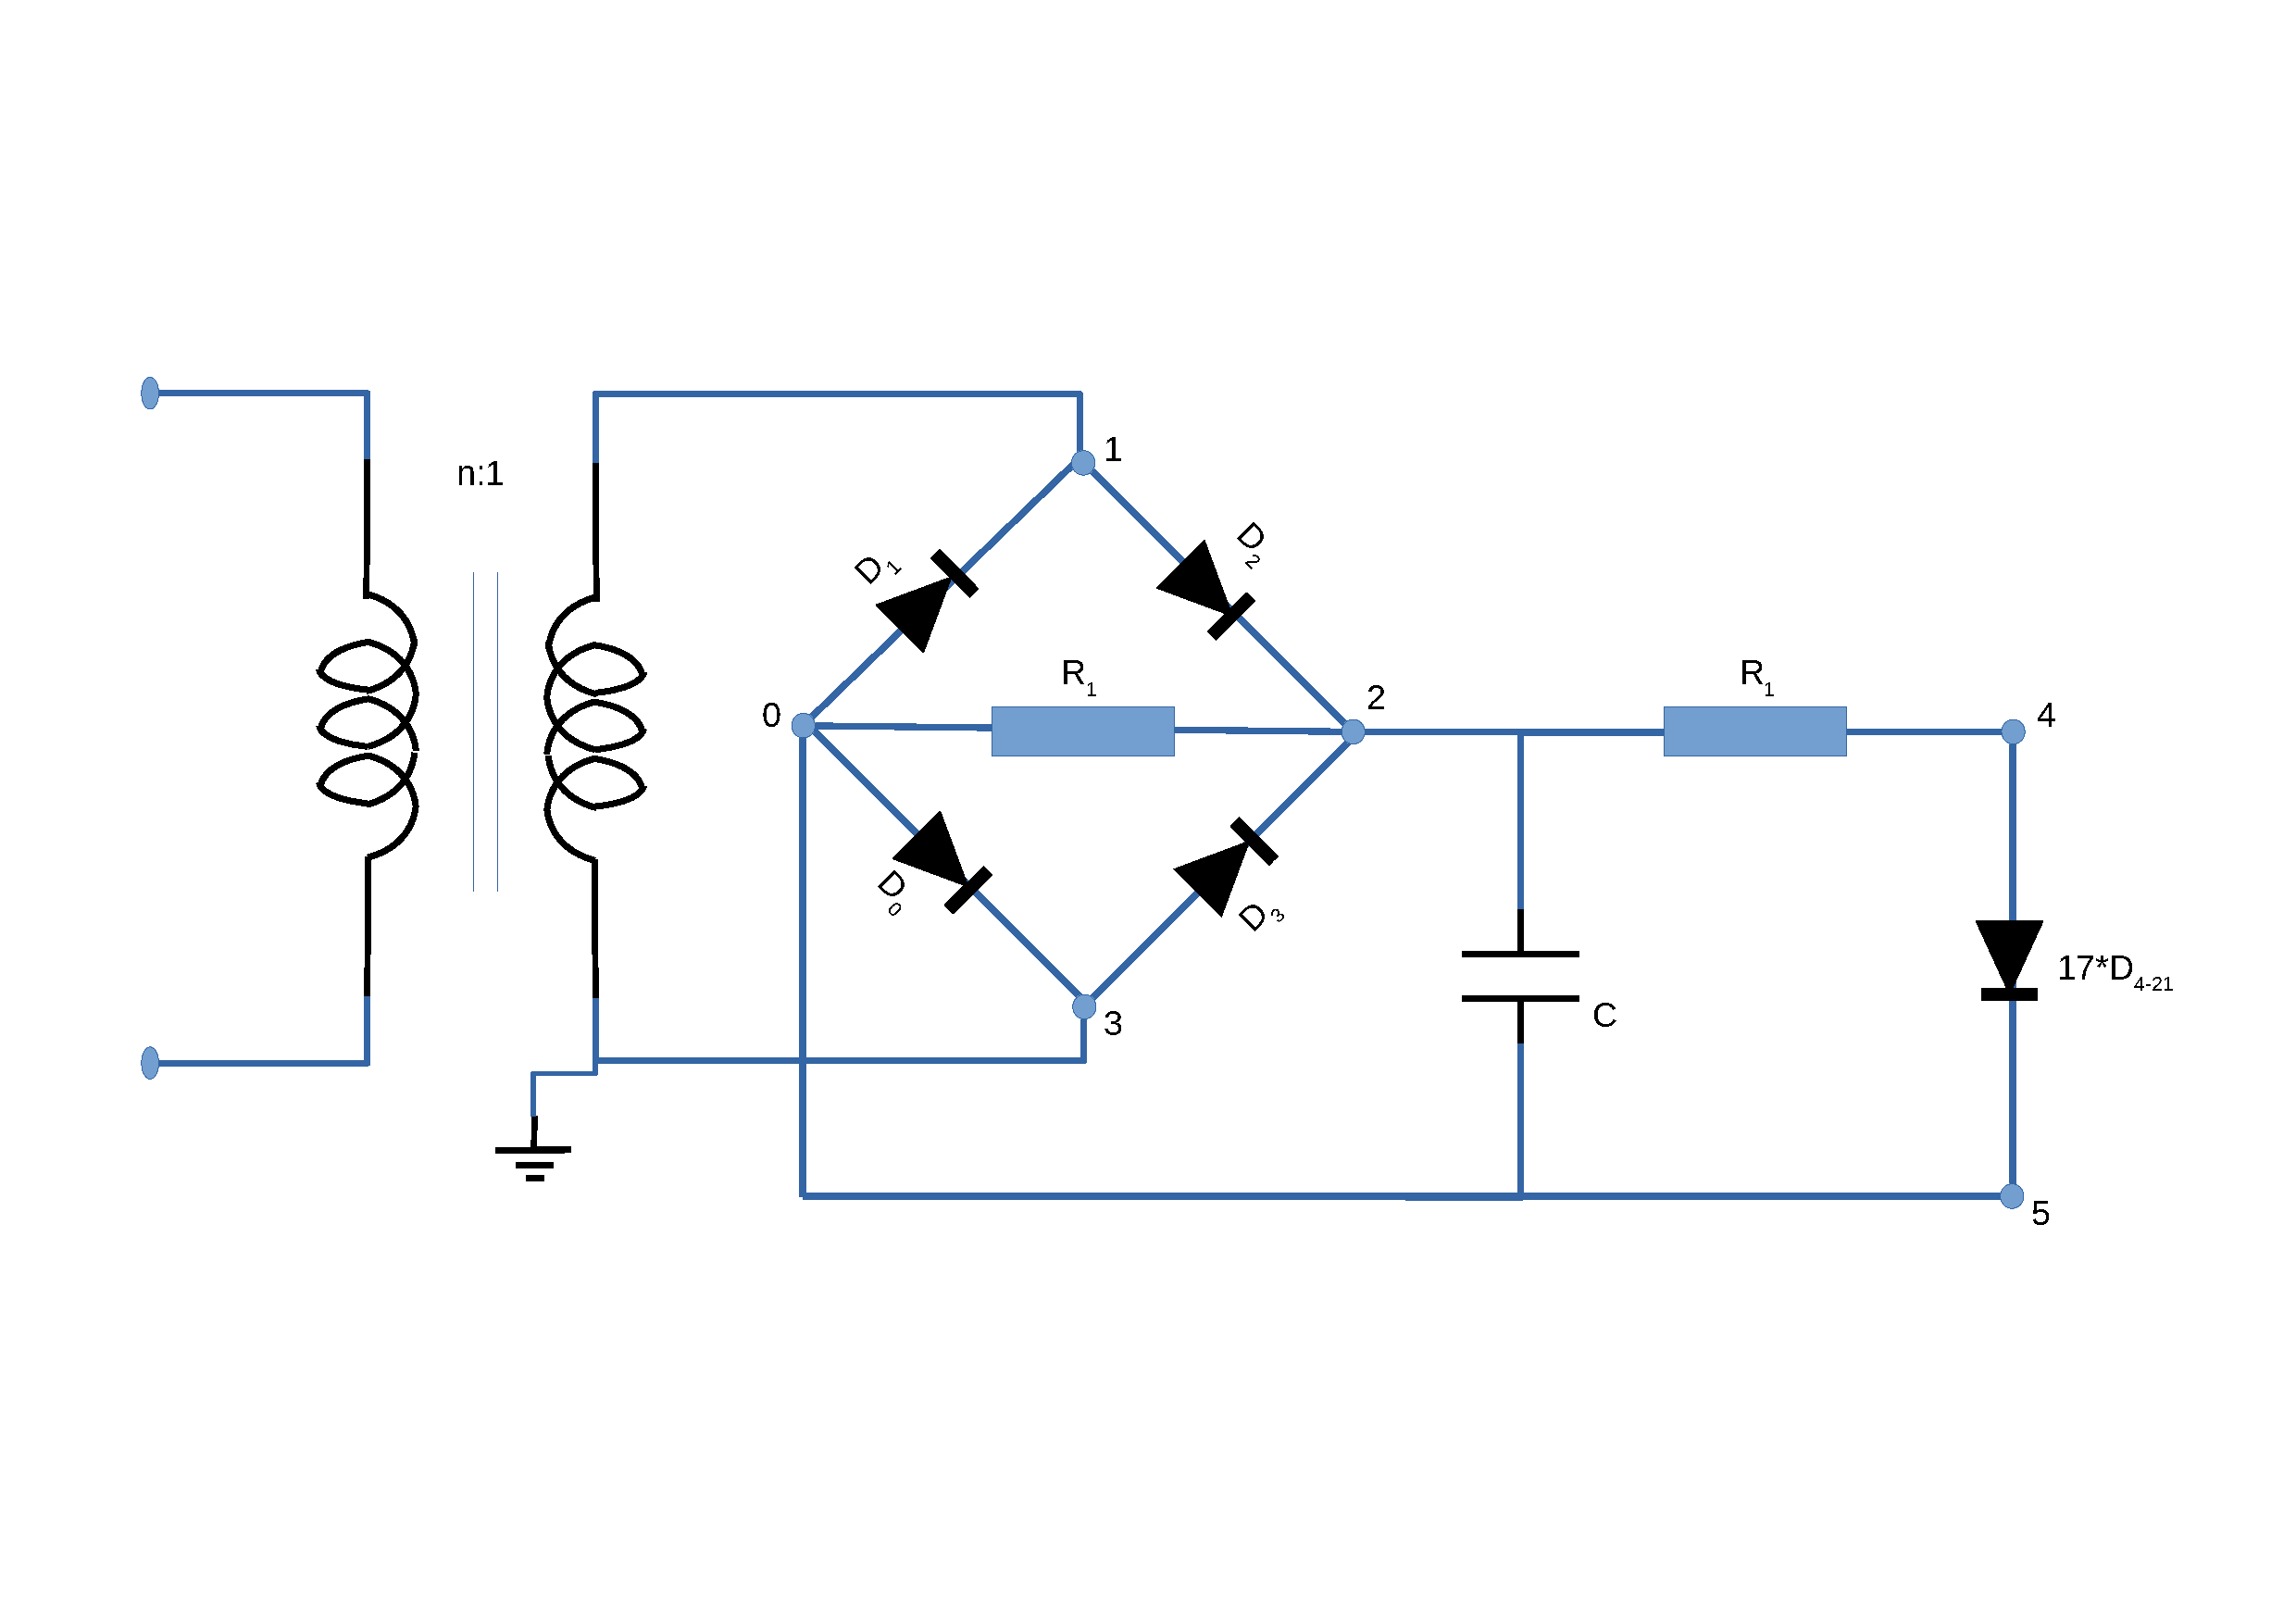
\includegraphics[width=0.9\textwidth, scale=1.0]{DesenhoT3.pdf}
\squeezeup 
\squeezeup 
\squeezeup 
\squeezeup 
\label{fig:circuit}
\end{figure}

As mentioned above, it is also important to refer that we have developed an optimization algorithm (in Octave) in order to find the number of diodes, the values of the resistors and capacitor and the consequent "n" (relation established by the number of coils in each side of the transformer) that would lead to the best value of merit, computed in Ngspice with the formula given by the Professor.   

